\documentclass[12pt]{article}
\usepackage{hyperref}
\usepackage{amsmath}
%\usepackage{amsmath}
\usepackage{graphicx}


\title{Generation SM particles that subsequently decay into millicharged particles}

\author{C. Campagnari (UCSB), F. Golf (UNL), B. Marsh (UCSB)}

\begin{document}
\maketitle


\section{Introduction}
In this document we discuss the generation of SM particles that in 
a subsequent step will be made to decay into milliCharged particles.
The key features of our approach are the following
\begin{itemize}
\item Use theory or some MC to generate $P_T$ distributions for SM
  particles
saved as histograms in ROOT files (Drell Yan is an exception, see
discussion in Section~\ref{sec:DY}.
\item Sample the ROOT histograms to generate SM particles of a 
given $P_T$
\item Pick azimuthal angles $\phi$ and pseudorapity $\eta$ in a
  limited 
range, matched to the acceptance of milliqan.
\item Decay the SM particles into milliCharged particles (this 
step is described in a separate note).  
\item When possible, keep track of theoretical uncertainties.
\item In general it is sufficient to generate SM particles at low 
and moderate $P_T$ since that is where the cross-section is largest.
\end{itemize}

\section{Drell Yan}
\label{sec:DY}

Golf needs to fix his bugs.

\section{J/$\psi$ and $\psi'$ from b-decays}
\label{sec:bpsi}
We use the tool available in \\
\href{http://www.lpthe.jussieu.fr/~cacciari/fonll/fonllform.html}
{http://www.lpthe.jussieu.fr/~cacciari/fonll/fonllform.html} \\
to
generate histograms of $P_T$ distributions (cross-sections) for charmonium from 
bottom decays, including theoretical 
uncertainties\cite{Cacciari:2012ny,Cacciari:2015fta}.  
See Figure~\ref{fig:bpsi} 

\begin{figure}
  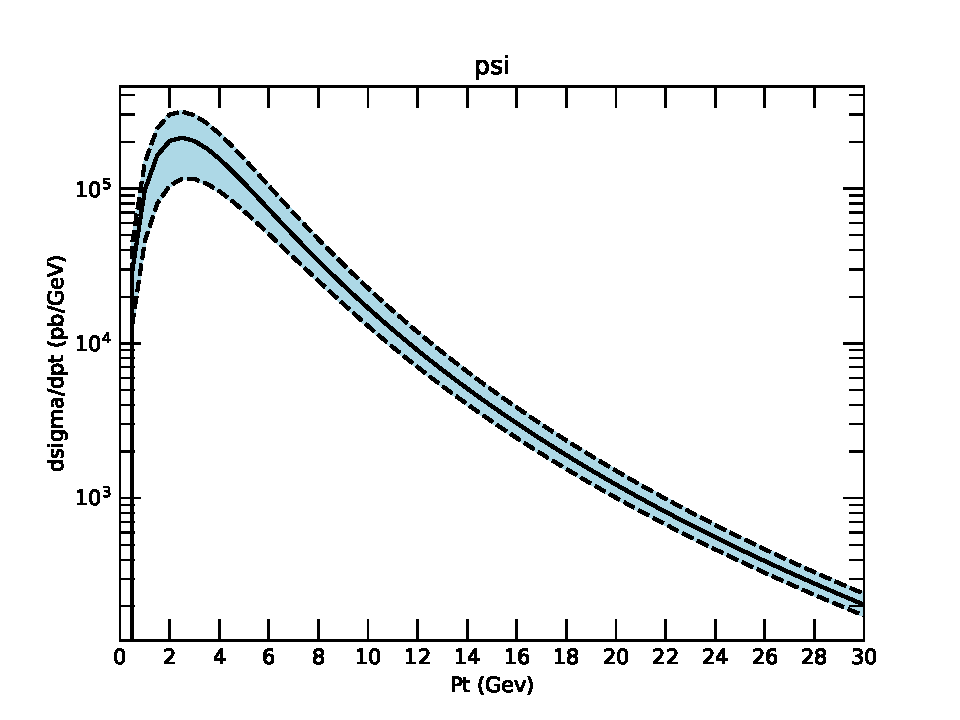
\includegraphics[width=0.48\linewidth]{../oniaFromB/psi.pdf}
  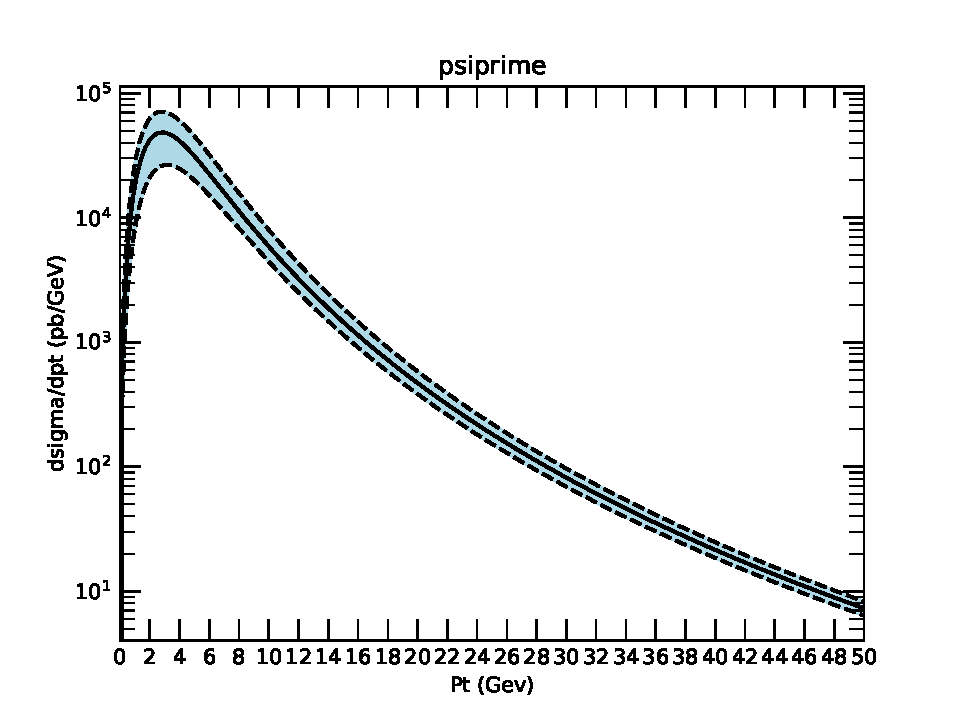
\includegraphics[width=0.48\linewidth]{../oniaFromB/psiprime.pdf}
  \caption{Transverse momentum distributions of J/$\psi$ (left) 
and $\psi'$ from bottom quark decays. Note: this is from a single $b$, 
multiply by two to include $\bar{b}$.}
  \label{fig:bpsi}
\end{figure}

\section{Direct onia production}
\label{sec:onia}

\noindent For charmonium I expect that the theorists I have been
communicating with
will give us distributions down to zero $P_T$, so we can do the same
thing that we did for charmonium.  However for bottmium they claim
that they cannot go below 15 GeV, so we need to figure out what to do.


\section{$\pi^0$, $\eta$, $\eta'$, $\phi$, $\rho$, and $\omega$}
\label{sec:mesons}

We generate these from Pythia.  The measurement of the 
$\pi^{\pm}$
$P_T$ spectrum from CMS\cite{Sirunyan:2017zmn} is in good agreement
with Pythia 8 Minimum Bias at low momentum.  We use this MC for all
mesons.  We do not attempt to use QCD $2 \to 2$ at very low $P_T$ since the 
process is infrared divergent.
Note that Pythia {\tt SoftQcd:nonDiffractive} includes all
hard QCD processes\cite{wwwPythia} so in principle this is all that is
needed.    However, one runs out of statistics at high $P_T$.  So 
at high $P_T$ we stitch together the minimum bias distributions with 
distributions obtained from QCD $2 \to 2$ at moderate $P_T$.

Eventually we will generate Pythia events in ``standalone'' mode to
be independent of CMS software.  For now we use existing CMS Monte
Carlos
for Minimum Bias and for QCD.  The CMS QCD samples are
``$P_T$-binned'',
(15-30 GeV, 30-50 GeV, and 50-80 GeV).  The Minimum Bias 
cross-section 
is taken to be 78.4 mb.  Then the stitching procedure is the following:
\begin{itemize}
\item The QCD samples are first normalized to their LO cross-sections.
\item next, we estimate a ``qcd-minbias scale factor'' by integrating
  over some region where the ratio is roughly flat
\item the QCD samples are renormalized by this scale factor
\item the samples are then stitched together by visually picking the 
$P_t$ where the curves cross each other.
\end{itemize}
\noindent The resulting $P_T$ curves are shown in
Figure~\ref{fig:mesons}.  It is not clear what kind of uncertainties
we should assign.  Let's first see how important these are at the end
of the day before going crazy.



\begin{figure}
  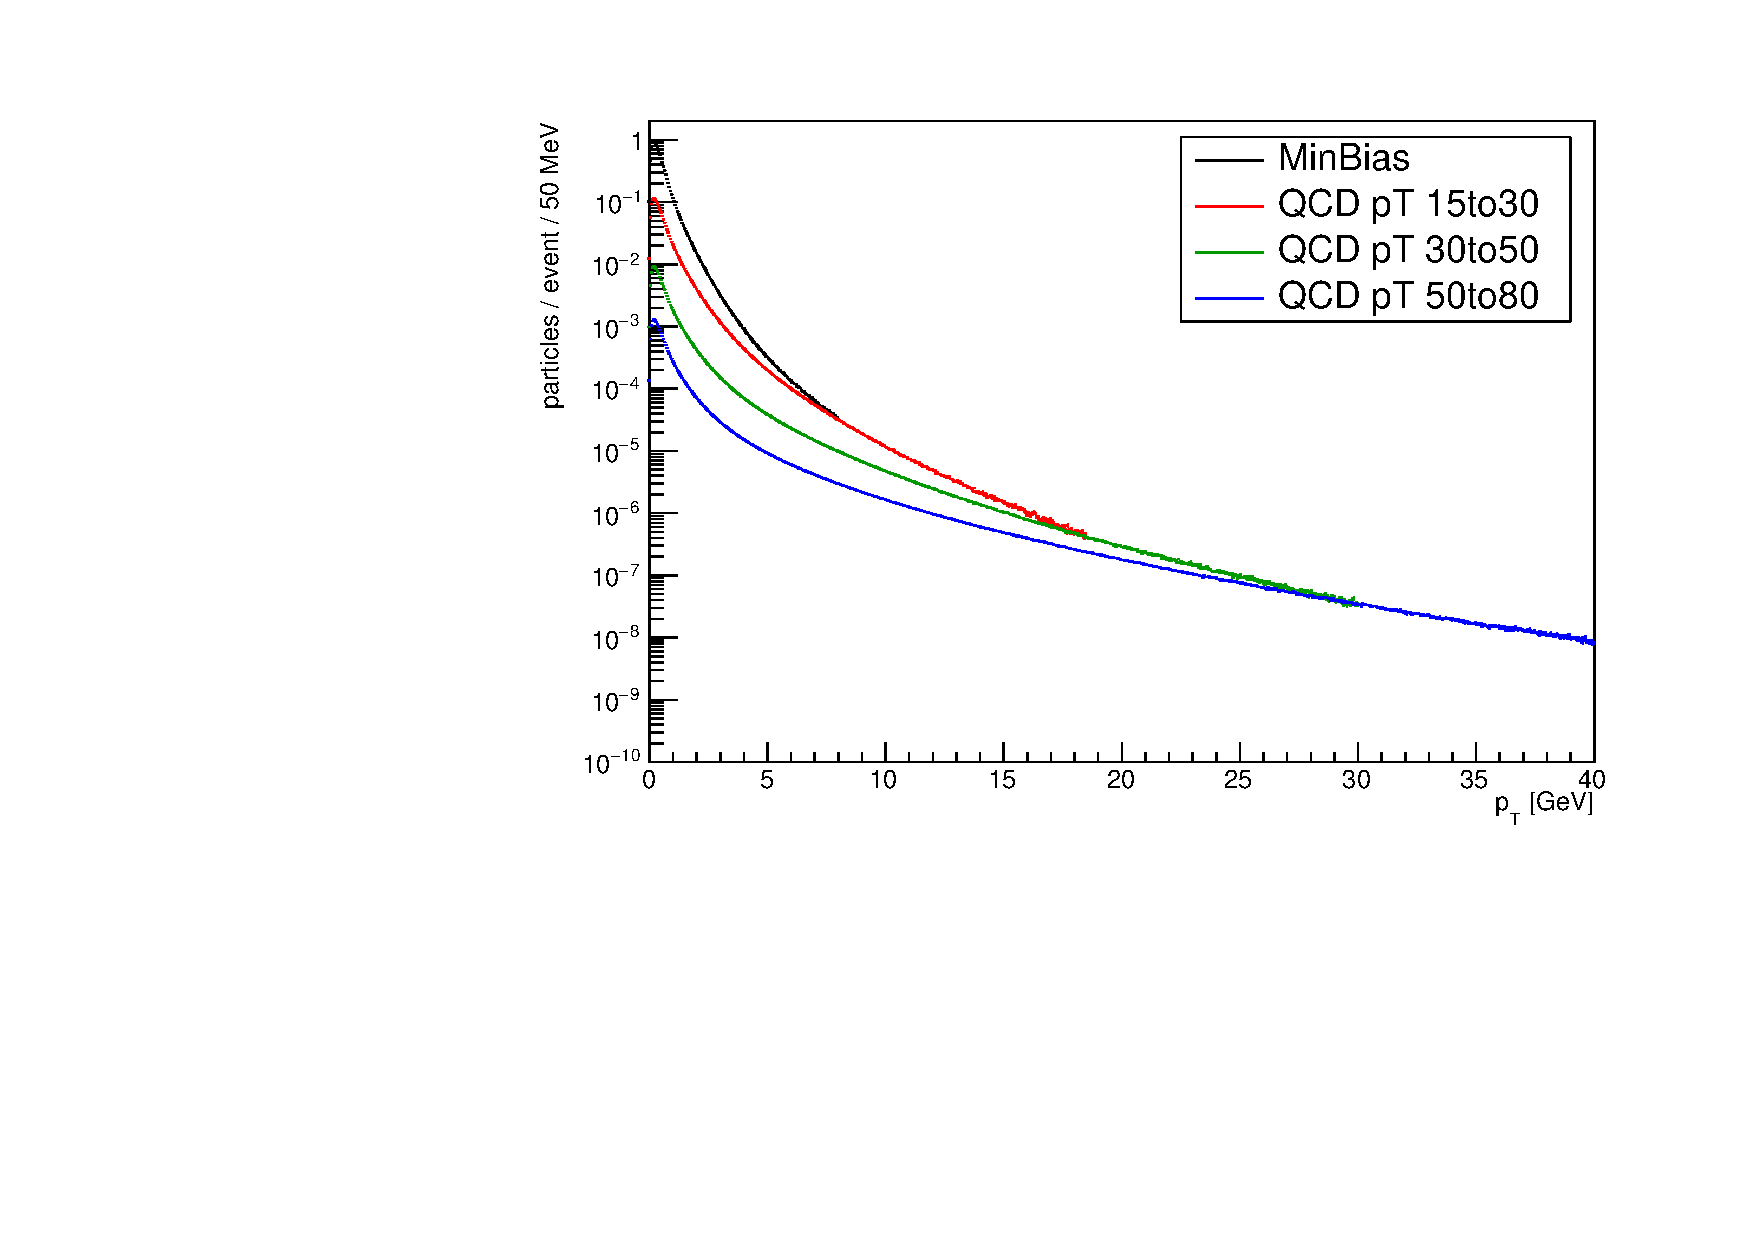
\includegraphics[width=0.48\linewidth]{plots/h_pi0.pdf}
  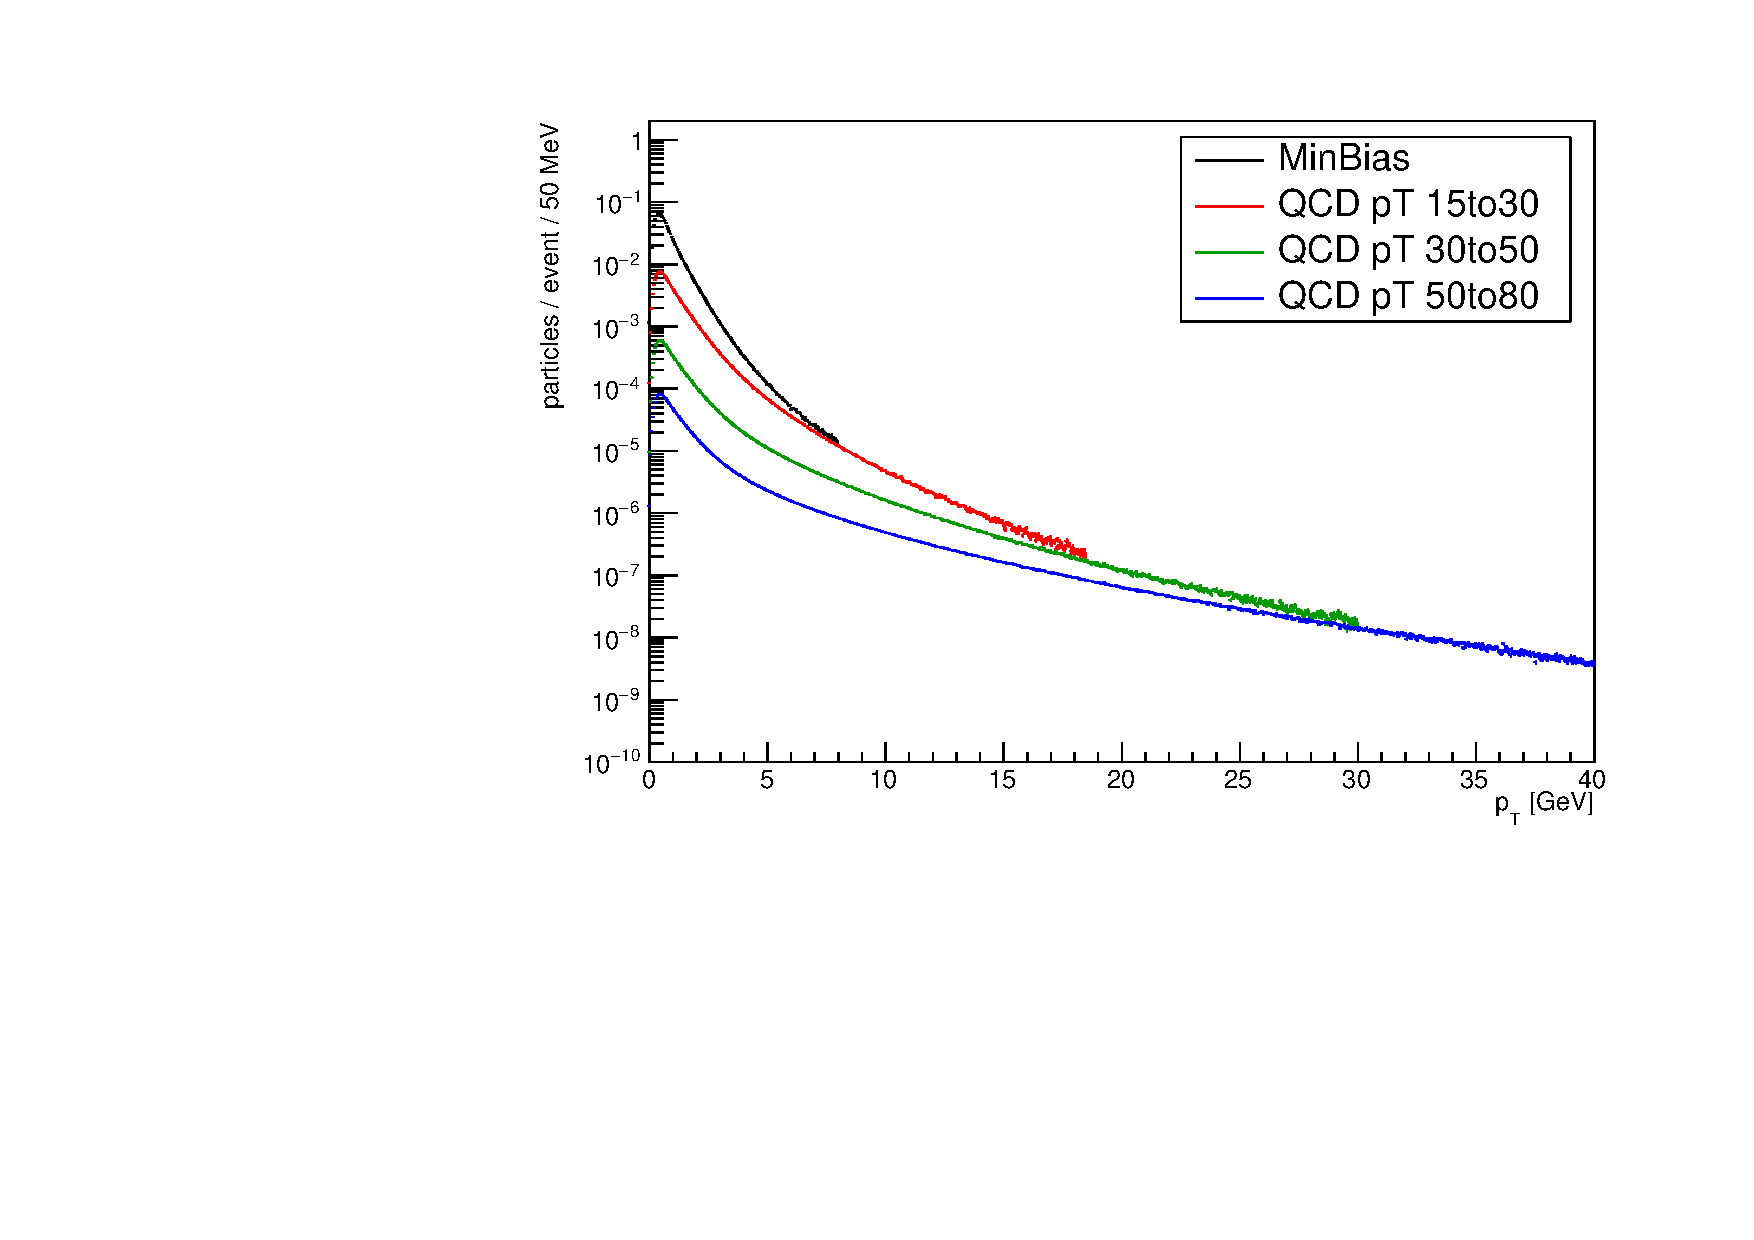
\includegraphics[width=0.48\linewidth]{plots/h_eta.pdf}
  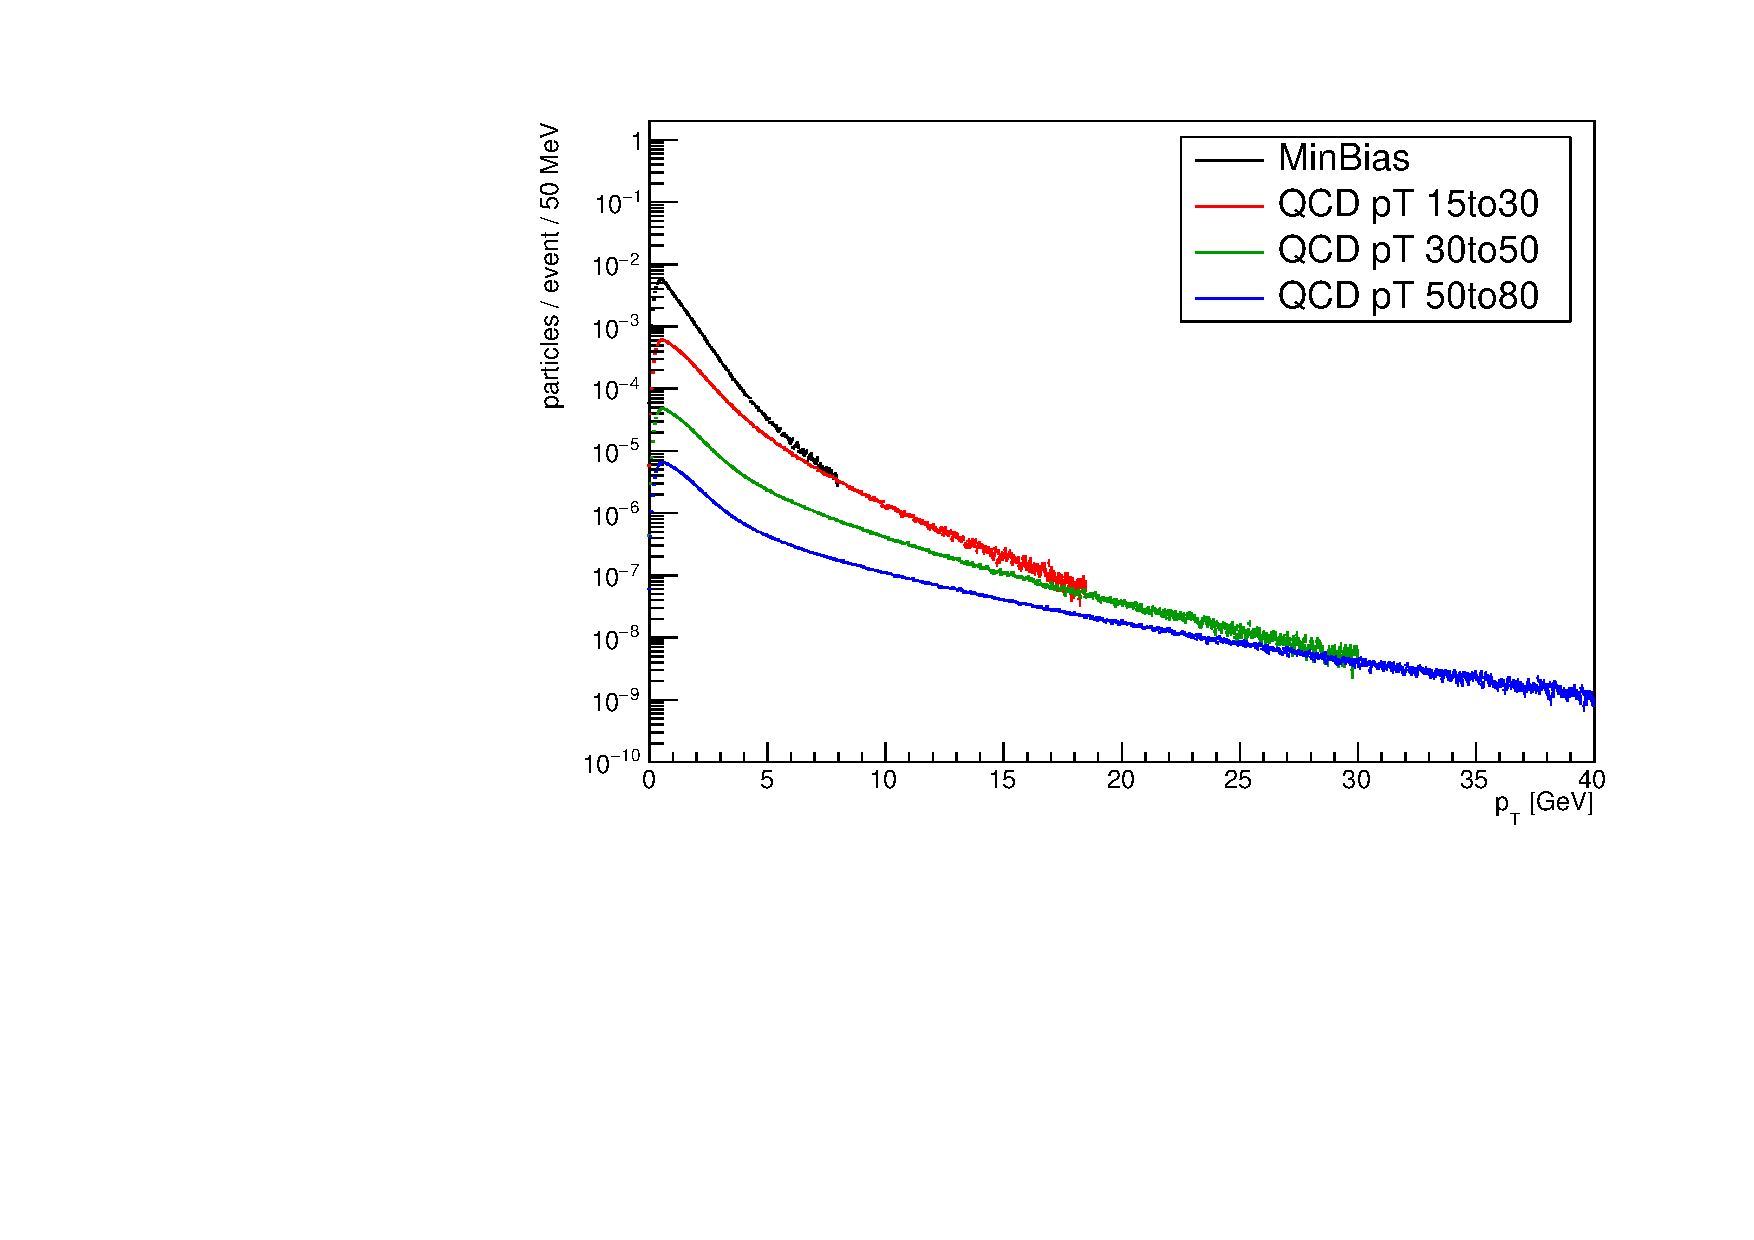
\includegraphics[width=0.48\linewidth]{plots/h_etap.pdf}
  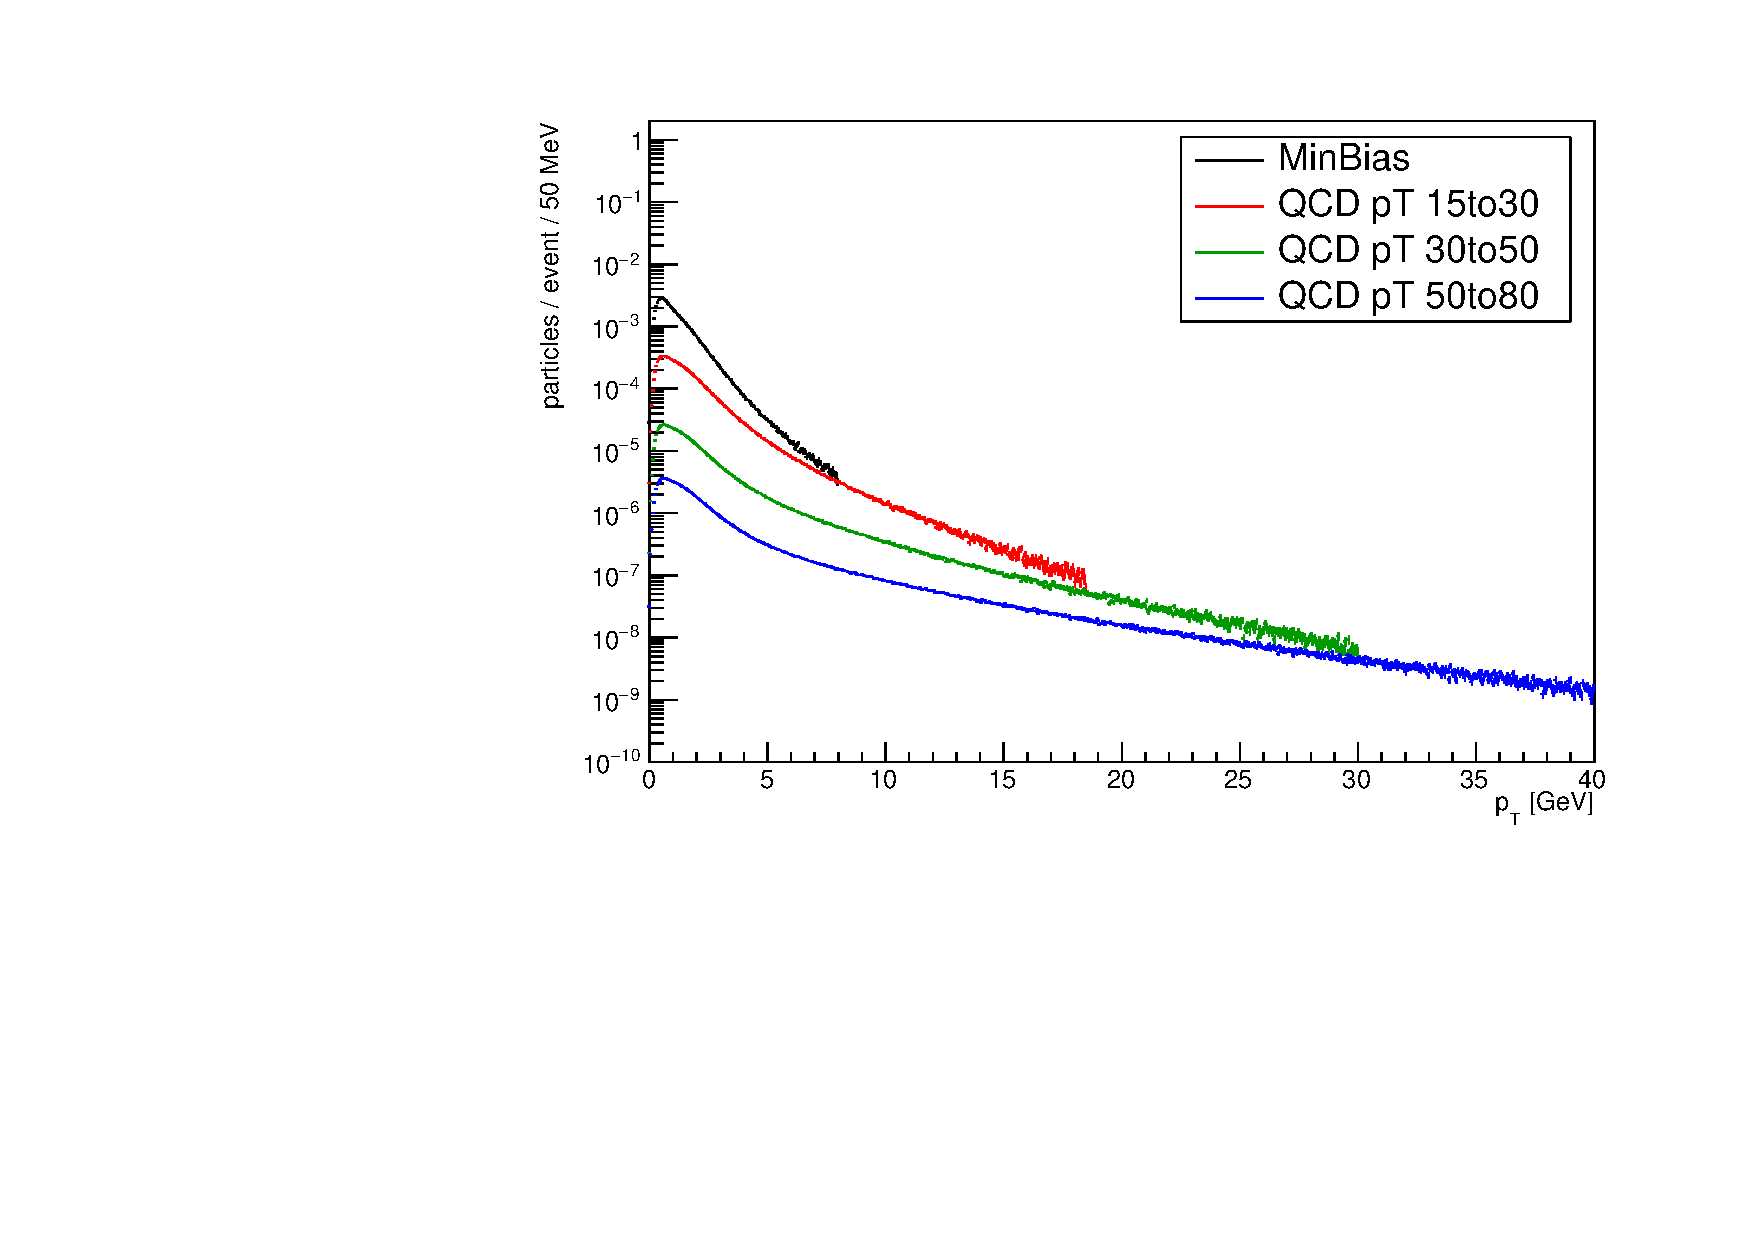
\includegraphics[width=0.48\linewidth]{plots/h_phi.pdf}
  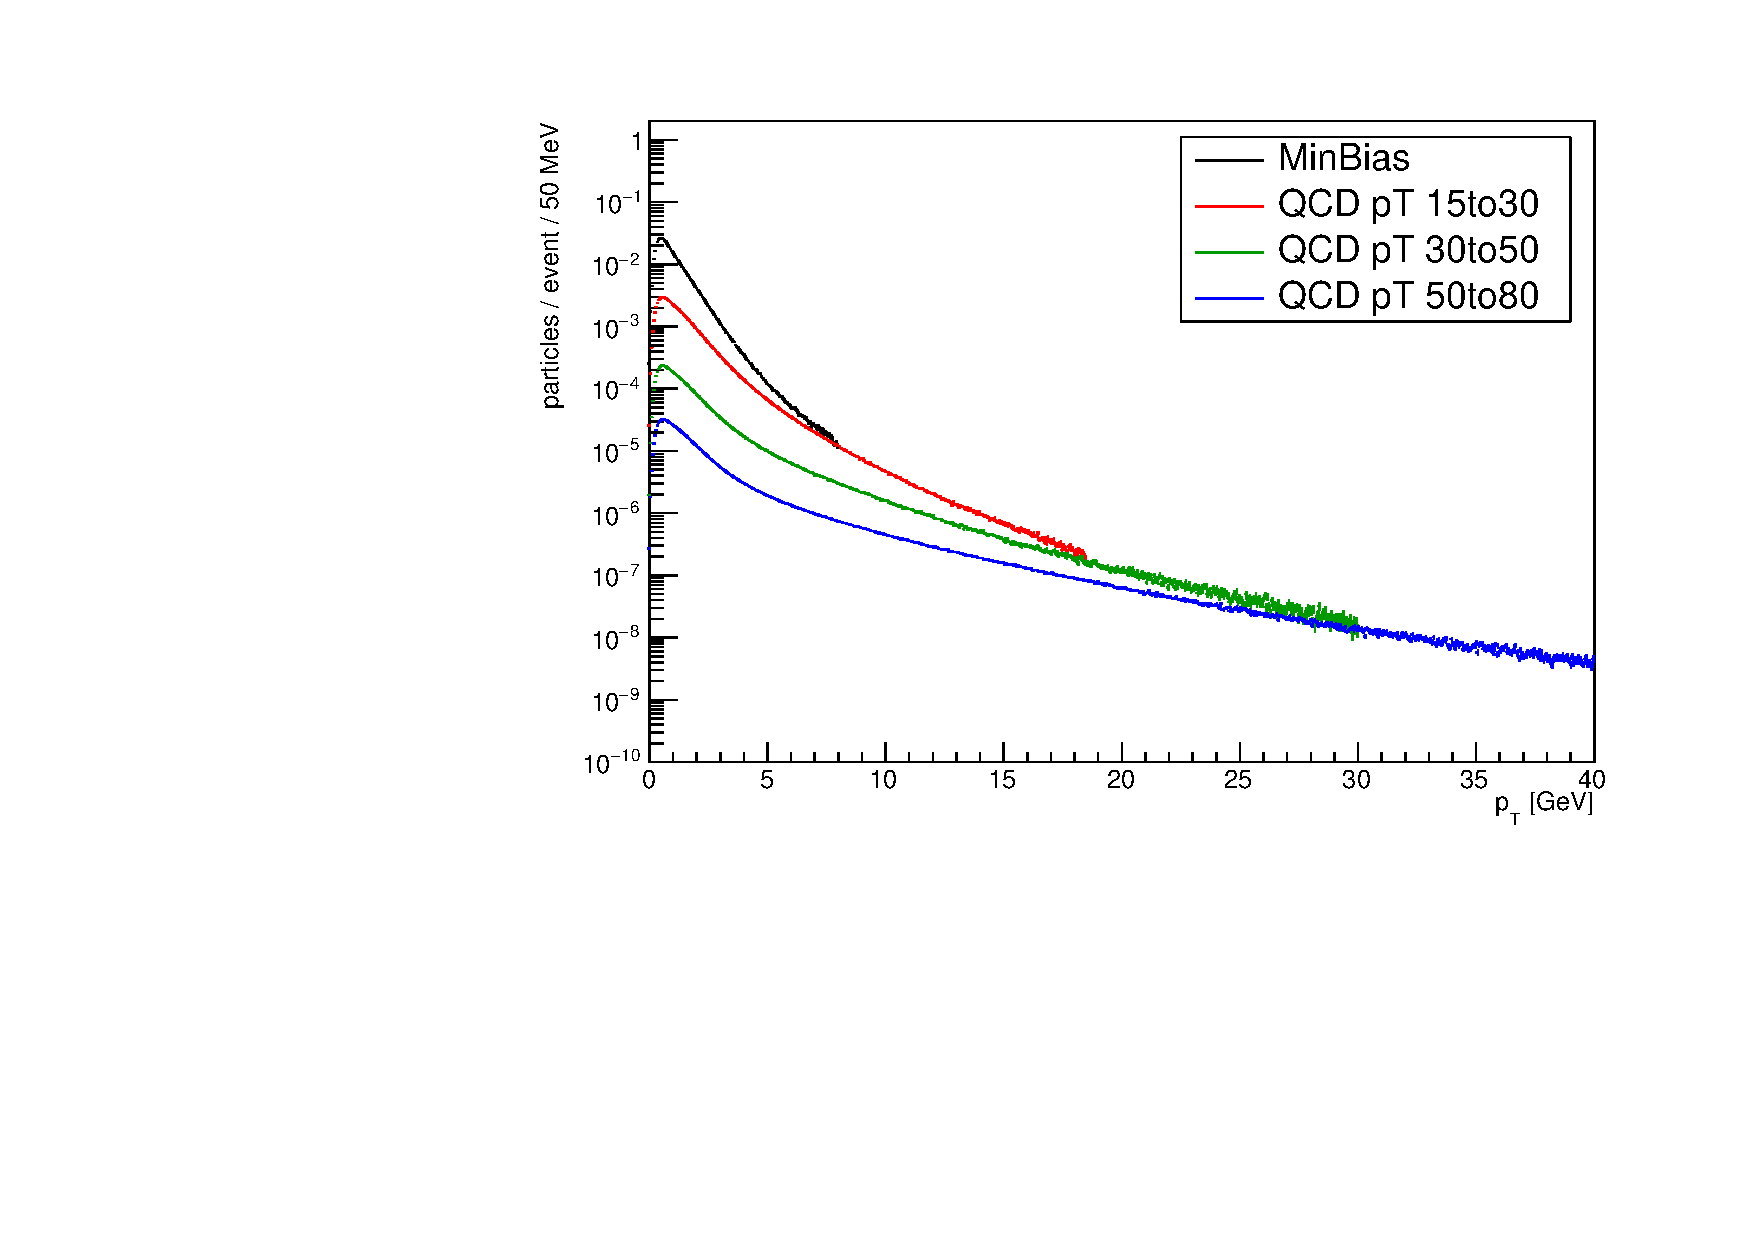
\includegraphics[width=0.48\linewidth]{plots/h_rho.pdf}
  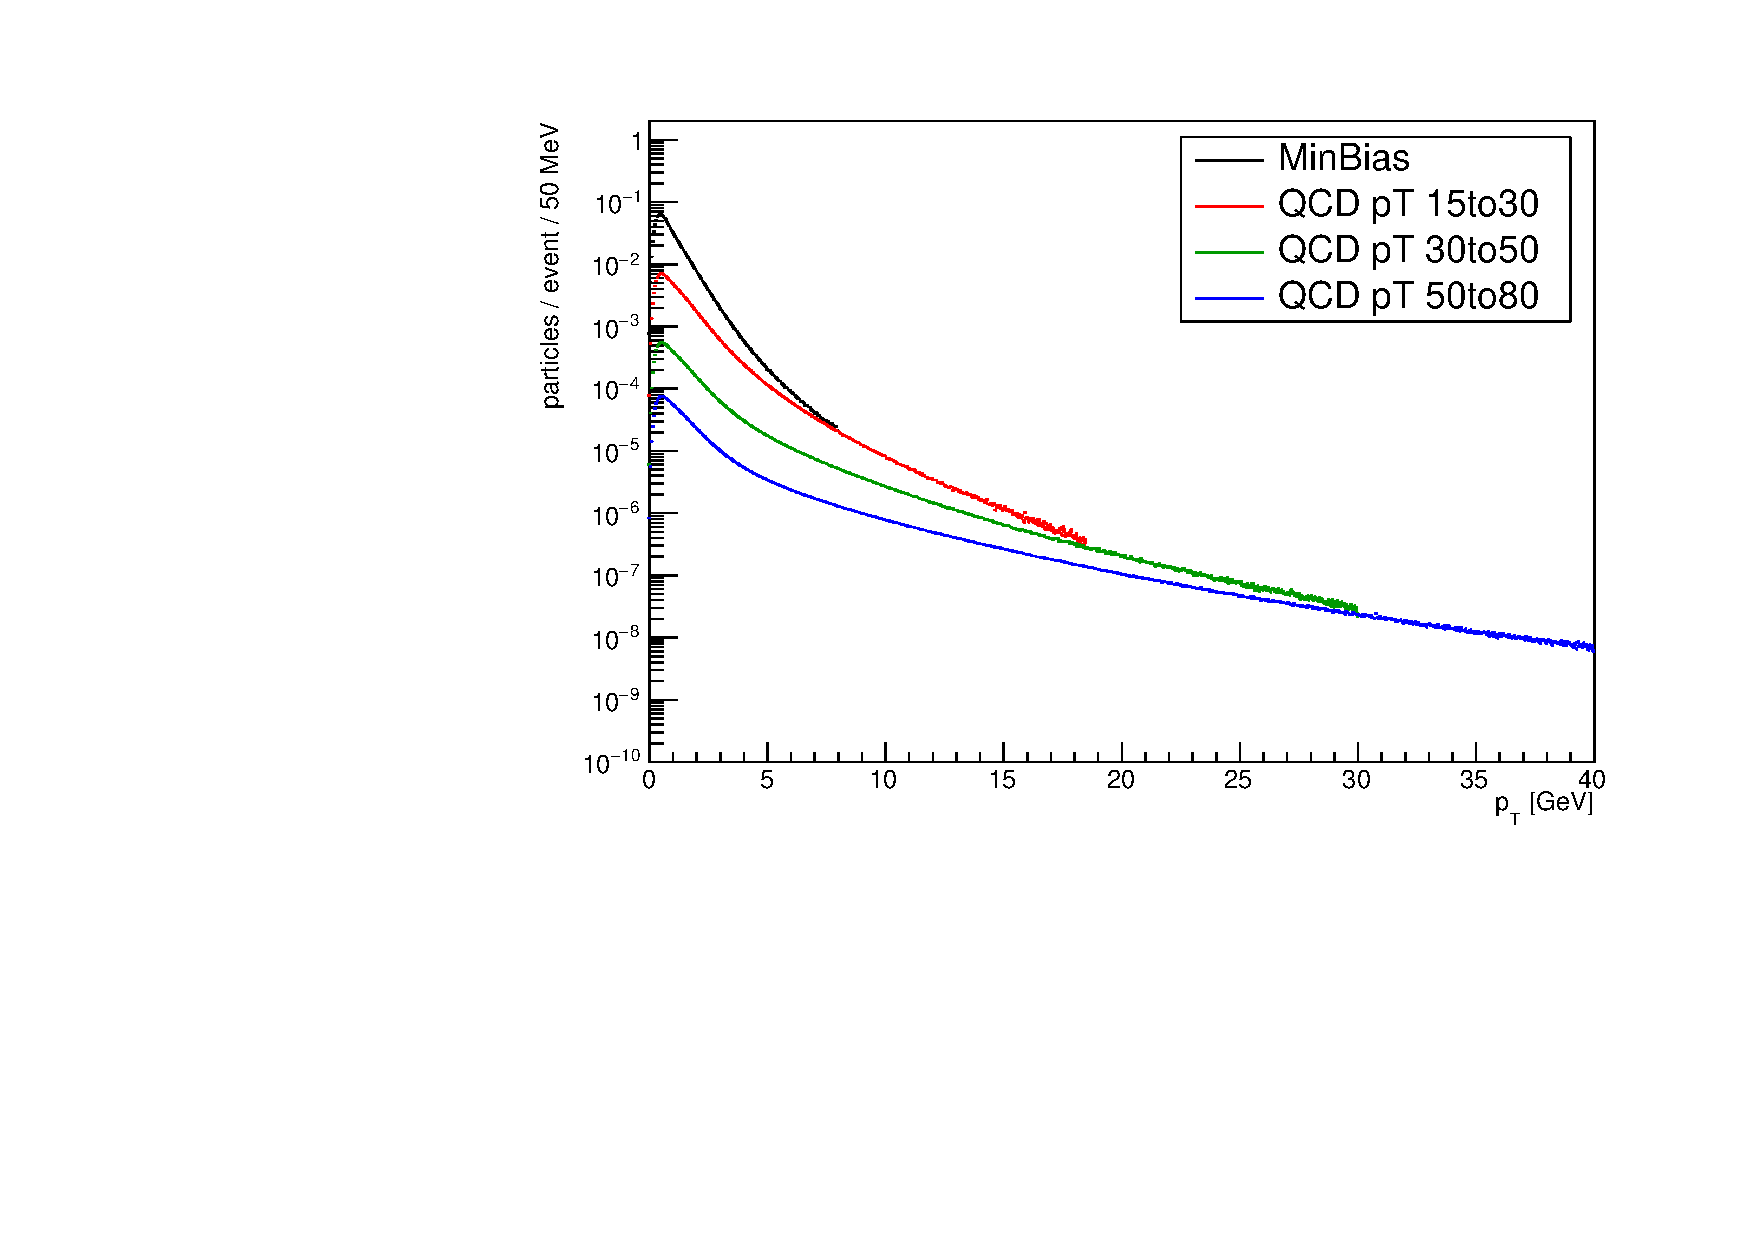
\includegraphics[width=0.48\linewidth]{plots/h_omega.pdf}
  \caption{\protect Transverse momentum distributions of 
$\pi^0$, $\eta$, $\eta'$, $\phi$, $\rho$, and $\omega$, top left
to bottom right, for $|\eta| < 1$.}
\label{fig:mesons}
\end{figure}



\begin{thebibliography}{1}

%\cite{Cacciari:2012ny,Cacciari:2015fta}
\bibitem{Cacciari:2012ny}
  M.~Cacciari, S.~Frixione, N.~Houdeau, M.~L.~Mangano, P.~Nason and G.~Ridolfi,
  % ``Theoretical predictions for charm and bottom
  % production at the LHC,''
  JHEP {\bf 1210} (2012) 137 [arXiv:1205.6344 [hep-ph]].
  %%CITATION = ARXIV:1205.6344;%%

\bibitem{Cacciari:2015fta}
  M.~Cacciari, M.~L.~Mangano and P.~Nason,
  %``Gluon PDF constraints from the ratio of forward heavy quark production at
  % the LHC at \sqrt{S}=7 and 13 TeV,''
  arXiv:1507.06197 [hep-ph].
  %%CITATION = ARXIV:1507.06197;%%

\bibitem{Sirunyan:2017zmn} 
  A.~M.~Sirunyan {\it et al.} [CMS Collaboration],
  %``Measurement of charged pion, kaon, and proton production in proton-proton collisions at $\sqrt{s}=13$ TeV,''
  Phys.\ Rev.\ D {\bf 96}, no. 11, 112003 (2017)
  doi:10.1103/PhysRevD.96.112003
  [arXiv:1706.10194 [hep-ex]].
  %%CITATION = doi:10.1103/PhysRevD.96.112003;%%
  %25 citations counted in INSPIRE as of 20 Jun 2019

\bibitem{wwwPythia}
\href{http://home.thep.lu.se/\~torbjorn/pythia81php/Welcome.php}
{http://home.thep.lu.se/\~torbjorn/pythia81php/Welcome.php}.  Click on 
{\tt QCD} on th eleft panel.

\end{thebibliography}  
\end{document}
